\documentclass[main.tex]{subfiles}
\begin{document}
\begin{enumerate}

\item À l'extérieur du carré, $f_{XY}(x,y) = 0$. À l'intérieur, le couple ($X,Y$) est uniformément réparti donc :
\[ f_{XY}(x,y) = 
\left\{ 
\begin{array}{ll}
\frac{1}{a^2} & \si x\in[0,a[, y\in[0,a[ \\
0 & \sinon
\end{array}
\right.
\]
$f_{XY}(x,y) = g_X(x)g_Y(x)$, $f_{XY}$ est séparable donc $X$ et $Y$ sont indépendantes.

\item On considère la VA $Z = X + Y$. Comme $X\in[0,a[$ et $Y\in[0,a[$, $Z\in[0,2a[$

Calculons la fonction de répartition de la VA Z.
\begin{align*}
F_Z(z) & = 
\left\{
\begin{array}{ll}
1 & \si z > 2a \\
? & \si z \in [0,2a] \\
0 & \si z < 0
\end{array}
\right.\\
\intertext{Si $z\in[0,2a[$, l'expression de la fonction de répartition n'est pas immédiate :}
F_Z(z) & = P[Z<z]  \\
& = P[(X,Y) \in D_z] \\
& = 
\left\{
\begin{array}{ll}
\frac{z^2/2}{a^2} & \si z\in[0,a] \\
\frac{a^2-\frac{(2a-z)^2}{2}}{a^2} & \si z\in[a,2a]
\end{array}
\right.
\end{align*}

\begin{center}
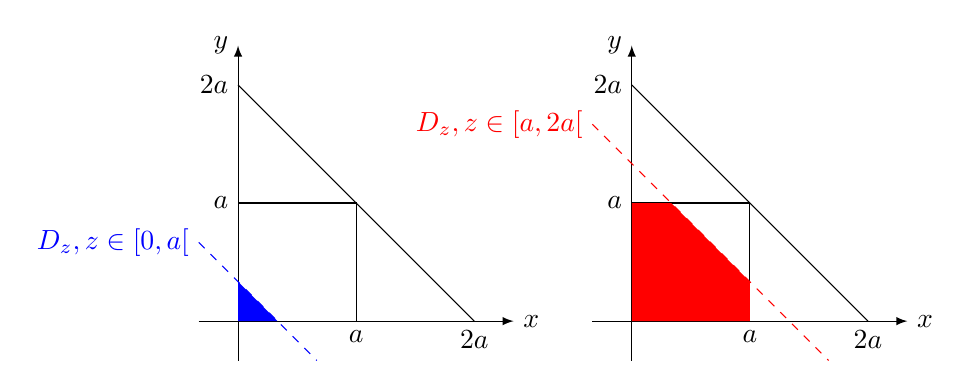
\begin{tikzpicture}[scale=0.5]
\draw [>=latex,->] (-1,0) -- (7,0) node[right]{$x$} ;
\draw [>=latex,->] (0,-1) -- (0,7) node[left]{$y$};

\draw (3,0) node[below]{$a$} -- (3,3) -- (0,3) node[left]{$a$};
\draw [dashed,blue] (-1,2) node[left]{$D_z, z\in[0,a[$} -- (2,-1); 
\draw (0,6) node[left]{$2a$} -- (6,0) node[below]{$2a$};

\fill [color=blue] (0,1) -- (1,0) -- (0,0);

\draw [>=latex,->] (9,0) -- (17,0) node[right]{$x$} ;
\draw [>=latex,->] (10,-1) -- (10,7) node[left]{$y$};

\draw (13,0) node[below]{$a$} -- (13,3) -- (10,3) node[left]{$a$};
\draw [dashed,red] (9,5) node[left]{$D_z, z\in[a,2a[$} -- (15,-1); 
\draw (10,6) node[left]{$2a$} -- (16,0) node[below]{$2a$};

\fill [color=red] (10,3) -- (11,3) -- (13,1) -- (13,0) -- (10,0);

\end{tikzpicture}
\end{center}

On peut donc résumer les résultats comme suit :
\begin{multicols}{2}
\[F_Z(z) = 
\left\{
\begin{array}{ll}
0 & \si z < 0 \\
\frac{z^2/2}{a^2} & \si z\in[0,a] \\
\frac{a^2-\frac{(2a-z)^2}{2}}{a^2} & \si z\in[a,2a] \\
1 & \si z > 2a 
\end{array}
\right.
\]

\[f_Z(z) =
\left\{
\begin{array}{ll}
0 & \si z < 0 \text{ ou } z > 2a \\
\frac{z}{a^2} & \si z\in[0,a] \\
\frac{2a-z}{a^2} & \si z\in[a,2a] 
\end{array}
\right.
\]
\end{multicols}

\begin{center}
\begin{tikzpicture}[scale=1]
\draw [>=latex,<->] (5,0) node[right]{$z$} -- (0,0) -- (0,2) node[left]{$f_Z(z)$};

\draw (0,0) node[below]{$0$} -- (2,1) -- (4,0) node[below]{$2a$};
\draw [dashed] (0,1) node[left]{$1/a$} -- (2,1) -- (2,0) node[below]{$a$};
\end{tikzpicture}
\end{center}

\item On commence par expliciter $F_Z(z)$ en fonction de $f_{XY}(x,y)$ :
\begin{align*}
F_Z(z) & = P[Z<z]  = \int_{-\infty}^z f_Z(w)dw \\
& = P[(X,Y) \in D_z] \\
& = \int \int_{D_z} f_{XY}(x,y)dxdy \\
F_Z(z) & = \int_ {-\infty}^{+\infty} ( \int_{-\infty}^{z-x} f_{XY}(x,y)dy)dx 
\end{align*}

\begin{center}
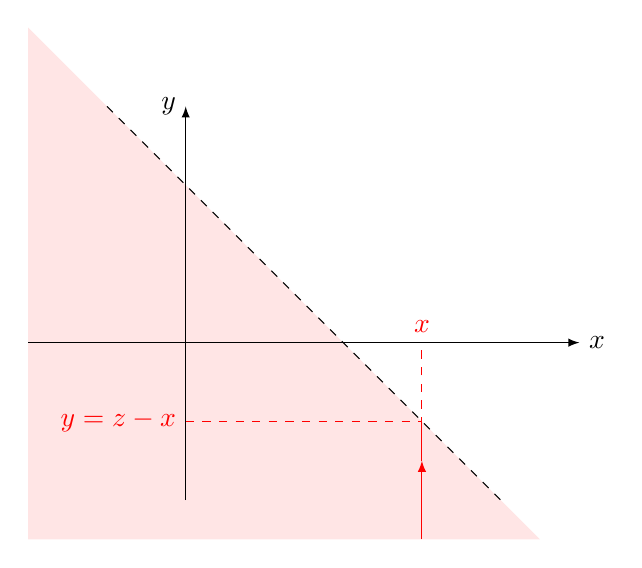
\begin{tikzpicture}[scale=1]
\fill [color=red!10] (4.5,-2.5) -- (-2,4) -- (-2,-2.5);

\draw [>=latex,->] (-2,0) -- (5,0) node[right]{$x$} ;
\draw [>=latex,->] (0,-2) -- (0,3) node[left]{$y$};

\draw [dashed] (-1,3) -- (4,-2);

\draw [>=latex,->,red] (3,-2.5) -- (3,-1.5);
\draw [red] (3,-1.5) -- (3,-1) ;
\draw [dashed, red] (0,-1) node[left]{$y=z-x$} -- (3,-1) -- (3,0) node[above]{$x$};
\end{tikzpicture}
\end{center}

On en déduit $f_Z(z)$ 
\begin{align*}
f_Z(z) & = \frac{dF_Z(z)}{dz} =  \frac{d}{dz} \int_ {-\infty}^{+\infty} ( \int_{-\infty}^{z-x} f_{XY}(x,y)dy)dx \\
& = \int_ {-\infty}^{+\infty} \frac{\partial}{\partial z} ( \int_{-\infty}^{z-x} f_{XY}(x,y)dy)dx \\
f_Z(z) & = \int_ {-\infty}^{+\infty} f_{XY}(x,z-x)dx
\end{align*}

\item Les VA $X$ et $Y$ indépendantes donc la ddp $f_{XY}(x,y)$ est séparable :
\begin{align*}
f_Z(z) & = \int_ {-\infty}^{+\infty} f_{XY}(x,z-x)dx \\
 & = \int_{-\infty}^{+\infty} f_X(x)f_Y(z-x)dx \\
f_Z(z) & = (f_X * f_Y)(z)
\end{align*}

\item Par définition de la fonction caractéristique de la VA $Z$ :
\begin{align*}
\phi_Z(u) & = E[e^{juZ}] \\
& = \int_{\mathbb{R}} f_Z(z) e^{juz} dz \\
\intertext{Ainsi, on peut réécrire }
\phi_Z(u) & = TF[f_Z(z)]_{f=-\frac{u}{2\pi}} \\
& = E[e^{ju(X+Y)}] = E[e^{juX}e^{juY}] \\
\intertext{Et par indépendance de $X$ et $Y$,}
\phi_Z(u) & = \phi_X(u)\phi_Y(u) \\
f_Z(z) &  = TF^{-1}[\phi_Z(u)](z) \\
& = (TF^{-1}[\phi_X(u)] * TF^{-1}[\phi_Y(u)])(z) \\
f_Z(z) & =(f_X * f_Y)(z)
\end{align*}

\item $X_1,...X_n$ indépendantes dans leur ensemble 
\begin{eqnarray*}
Y_{12} = & X_1 + X_2 & \rightarrow f_{Y_{12}}(y) = (f_{X_1}*f_{X_2})(y) \\
Y_{123} = & X_1 + X_2 + X_3 = Y_{12} + X_3 & \rightarrow f_{Y_{123}}(y) = (f_{Y_{12}} * f_{X_3})(y) = (f_{X_1}*f_{X_2}*f_{X_3})(y)
\end{eqnarray*}
Par récurrence, on montre alors que pour $Y = X_1 + ... + X_n$,
\[f_Y(y) = (f_{X_1}* ... * f_{X_n})(y) \]


On montre que pour $X_n, n=1,...,N$ VA réelles et scalaires indépendantes et identiquement distribuées, centrées et d'écart-type $\sigma$,
\[Z_N = \frac{\sum_{n=1}^N X_n}{\sqrt{N}} \text{ tend vers une VA gaussienne quand N tend vers } +\infty \]

\item Par linéarité de l'espérance, et comme les variables $X_N$ sont centrées ($E[X_N] = 0$),
\[ E[Z_N] = E[\frac{\sum_{n=1}^N X_n}{\sqrt{N}}] = \frac{\sum_{n=1}^N E[X_n]}{\sqrt{N}} = 0 \]

De plus, 
\begin{align*}
\sigma_Z^2 & = E[(Z_N - m_{Z_N})^2] = E[Z_N^2] \\
& = \frac{1}{N} E[(\sum_{n=1}^N X_n)^2] \\
& = \frac{1}{N} E[ \sum_{n=1}^N X_n^2 + \sum_{i\neq j} X_iX_j] \\
& = \frac{1}{N} (\sum_ {n=1}^N E[X_n^2] + \sum_{i\neq j} E[X_iX_j]) \\
& = \frac{1}{N} \sum_{n=1}^N \sigma^2 \\
& = \sigma^2
\end{align*} 
\newpage
\item Deux personnes se donnent rendez-vous entre 18h et 19h. On associe aux deux instants d'arrivées deux VA X et Y indépendantes, de ddp uniforme sur l'intervalle [18,19].

On introduit la VA $\Delta = |Y-X|$. Calculons sa fonction de répartition.
\begin{align*}
F_{\Delta}(\delta) & = P[\Delta \leq \delta] \\
& = P[ |Y-X| \leq \delta ] \\
& = P[ Y-X \leq \delta \et X-Y \leq \delta ] \\
& = P[ Y \leq X + \delta \et Y \geq X - \delta ]
\end{align*}

\begin{figure}[h!]
\centering
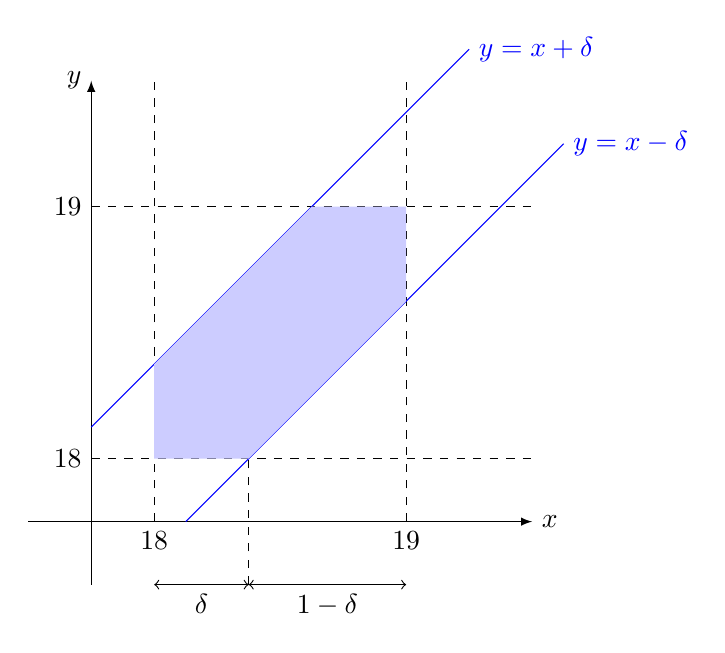
\begin{tikzpicture}[scale=0.8]
\draw [>=latex,->] (-1,0) -- (7,0) node[right]{$x$} ;
\draw [>=latex,->] (0,-1) -- (0,7) node[left]{$y$};

\draw [dashed] (1,0) node[below]{$18$} -- (1,7);
\draw [dashed] (5,0) node[below]{$19$} -- (5,7);
\draw [dashed] (0,1) node[left]{$18$} -- (7,1);
\draw [dashed] (0,5) node[left]{$19$} -- (7,5) ;

\draw [blue] (0,1.5) -- (6,7.5) node[right]{$y=x+\delta$};
\draw [blue] (1.5,0) -- (7.5,6) node[right]{$y=x-\delta$};

\fill [color=blue!20] (1,1) -- (1,2.5) -- (3.5,5) -- (5,5) -- (5,3.5) -- (2.5,1) -- (1,1);

\draw [dashed] (2.5,-1) -- (2.5,1);
\draw [<->] (1,-1) -- (2.5,-1);
\draw (1.75,-1) node[below]{$\delta$};
\draw [<->] (5,-1) -- (2.5,-1);
\draw (3.75,-1) node[below]{$1-\delta$};
\end{tikzpicture}
\end{figure}

Ainsi, \[F_{\Delta}(\delta) = 
\left\{
\begin{array}{ll}
0 & \si \delta < 0 \\
1 - (1-\delta)^2 & \si 0 \leq \delta < 1\\
1 & \si \delta \geq 1
\end{array}
\right.
\]

Donc \[f_{\Delta}(\delta) =
\left\{
\begin{array}{ll}
2 - 2 \delta & \si 0 \leq \delta < 1\\
0 & \sinon
\end{array}
\right.
\]

\end{enumerate}
\end{document}
